\chapter{Simulation}

This chapter presents the simulation framework developed to evaluate and 
compare task-priority control methods for light-UVMSs. The chapter begins by 
introducing the robot model, derived from the mathematical framework 
established in the previous chapter, and outlines the simulation environment 
and performance metrics. Different task-priority control strategies, both at 
the kinematic and dynamic levels, are implemented and tested in a series of 
simulation scenarios. The results provide insights into the performance, 
computational cost, and robustness of each approach, laying the groundwork for 
future experimental validation.

\iffalse
% -----------------------------------------------------------------------------
\section{Introduction}
\begin{itemize}
    \item Purpose of simulation.
    \item objective: Compare kinematic-level and dynamic-level controllers
    \item Highlight expected insights. performance, stability, robustness,
        computational cost?
\end{itemize}
This section should be very general. I don't want to give specifics on the
tasks and the specific types of controllers used.
\fi

% -----------------------------------------------------------------------------
\section{Simulation Setup}

\subsection{Robot Model}

% Present the Eelume 500 robot
% Describe the simplified model used in the simulation

The light-UVMS that will be used in the simulation is a simplified version of
the Eelume 500 robot. This decision was based on the goal to implement a physical
task-priority controller this robot in the future. The Eelume 500 robot is a
snake-like robot with 3 joints and 2 links.
A picture of the Eelume 500 robot is shown in Figure \ref{fig:eely}.

\begin{figure}[h!]
    \centering
    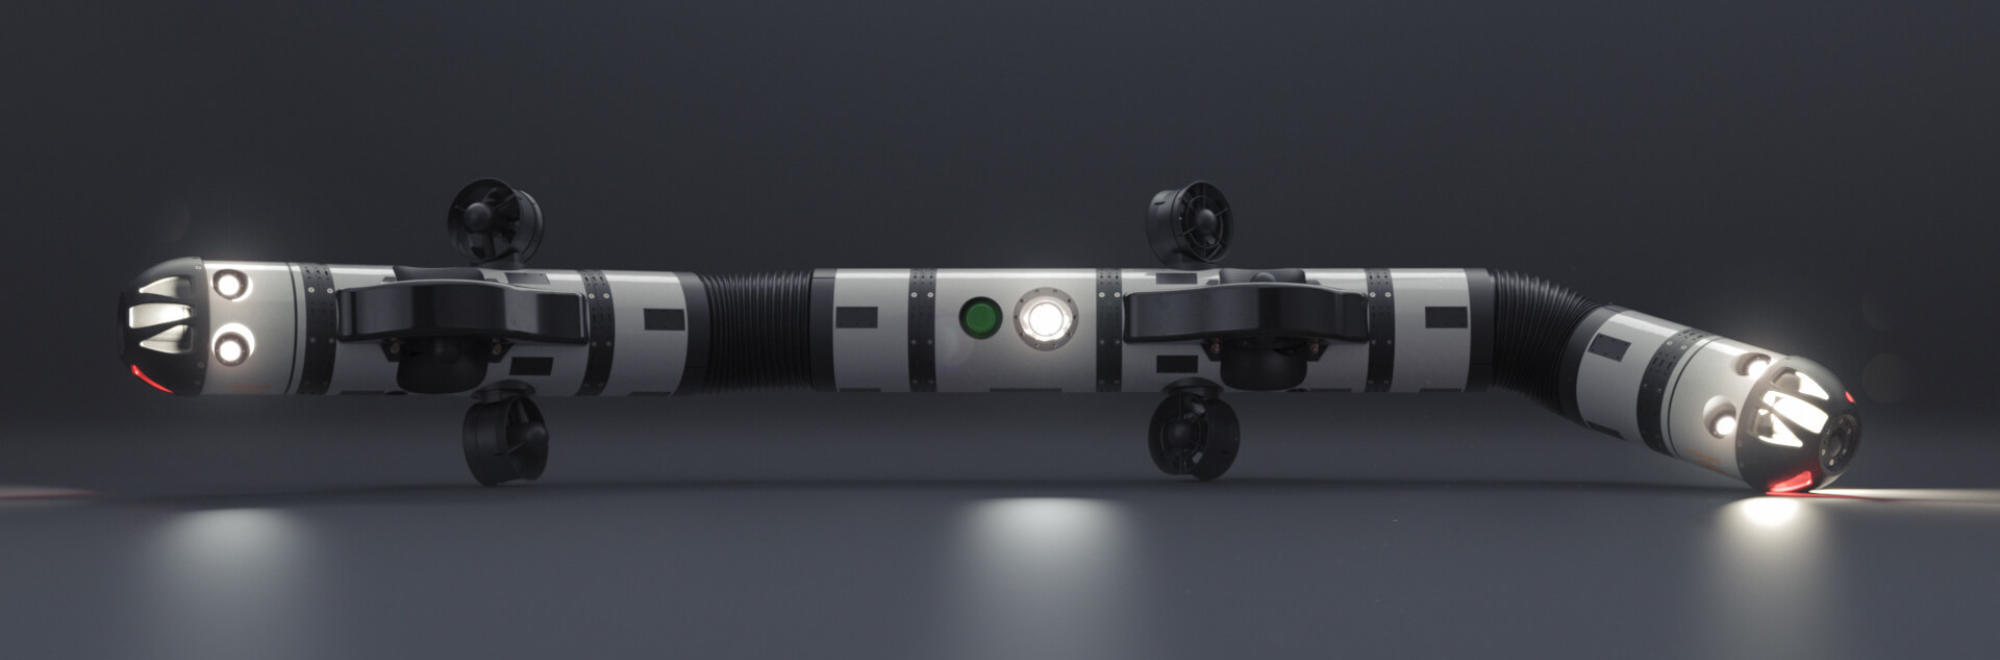
\includegraphics[width=0.8\linewidth]{assets/images/eely.jpg}
    \caption{Computer rendering of the Eelume 500 robot. Credit: Eelume.}
    \label{fig:eely}
\end{figure}

Each of the joints has two degrees of freedom and is actuated by a pair of
motors. In addition, two of the links are equipped with a set of $4$ thrusters.
The thruster configuration allows the robot to move in all directions, making
the robot fully actuated. Although one can define the base of the robot as any
link, in this work, we will define the base as the middle link. The position of
the Eeelume robot is uniquely determined by the position of this base and the 
two pairs of joint angles, making the robot a 10-DOF system. The two sets of 
$4$ thrusters, as well as the two pairs of motors controlling the joints, are 
all independently actuated, making the input space of the robot a 
12-dimensional space.

We will denote each of the links with a number from $1$ to $3$, where link $1$,
the "head" of the robot, is the smallest link situated in the rightmost position
in \autoref{fig:eely}. The parameters of the Eelume robot are given in a
NED coordinate system, where the head of the robot is the most northern point.

We will assume that the robot in neutrally buoyant. In reality, weights can be
added to a module to adjust its center of mass, making the weight of the robot
equal to the weight of the water it displaces. This can however be a difficult
task as the density of water can vary, and the weights needs to be placed at 
predetermined locations meaning that one cannot place the center of mass at an
arbitrary location.
The parameters of the robot are given in \autoref{tab:robot}.

\begin{table}[h]
    \centering
    \begin{tabular}{|c|c|c|c|}
        \hline
        Parameter & Value & Unit & Description \\ \hline
        $r$ & 0.1 & m & Radius of each link \\
        $m_1$ & 40 & kg & Mass of link $1$ \\
        $m_2$ & 90 & kg & Mass of link $2$ \\
        $m_3$ & 50 & kg & Mass of link $3$ \\
        $l_1$ & 1.0 & m & Length of link $1$ \\
        $l_2$ & 2.3 & m & Length of link $2$ \\
        $l_3$ & 1.5 & m & Length of link $3$ \\
        $l_{\mathrm{joint}}$ & 0.6 & m & Length of each joint \\
        $\beta$ & 0.1 & - & Damping parameter \\
        $\gamma$ & 0.2 & - & Damping parameter \\
        $v_{\mathrm{ref}}$ & 0.1 & m/s & Reference velocity for damping \\
        $C_D$ & 0.3 & - & Damping coefficient \\
        $\rho$ & 1025 & kg/m$^3$ & Density of water \\
        \hline
    \end{tabular}
    \caption{Parameters for the simplified Eelume 500 robot.}
    \label{tab:robot}
\end{table}

The $\beta$, $\gamma$, $v_{\mathrm{ref}}$ and $C_D$ parameters specify the damping
coefficients of the robot. The damping matrix the parameters specify is given in
\autoref{eq:damping_cyl}. These parameters are based on \cite{bendik}. Added mass
is computed based on \autoref{eq:ellipsoid_added_mass}.
The inertia matrix of the robot is approximated as a
cylinder with uniform density and is as follows:

\begin{align}
    \bm{I}_i &=
    \begin{bmatrix}
        \frac{m_i}{2} r^2 & 0 & 0 \\
        0 & \frac{m_i}{12} (3r^2 + l_i^2) & 0 \\
        0 & 0 & \frac{m_i}{12} (3r^2 + l_i^2)
    \end{bmatrix} &
    i &= 1, 2, 3.
\end{align}

The thruster configuration is similar to that of \autoref{fig:eely}. The exact
specifications of the position and orientation of the thrusters can be seen in
\autoref{tab:thrusters}.

\begin{table}[h]
    \centering
    \begin{tabular}{|c|c|c|c|c|c|c|}
        \hline
        Link & Number & Thruster & $x$ [m] & $y$, [m] & $z$, [m] & Direction \\ \hline
        $2$ & 1 & Starboard & $0.56725$ & $-0.174$ & $0$ & South-Up \\
        $2$ & 2 & Port & $0.56725$ & $0.174$ & $0$ & South-Down \\
        $2$ & 3 & Bottom & $0.67725$ & $0.000$ & $0.09$ & East \\
        $2$ & 4 & Top & $0.67725$ & $0.000$ & $-0.09$ & West \\ \hline
        $3$ & 5 & Starboard & $0.02025$ & $-0.174$ & $0$ & South-Down \\
        $3$ & 6 & Port & $0.02025$ & $0.174$ & $0$ & South-Up \\
        $3$ & 7 & Bottom & $-0.08975$ & $0.000$ & $0.09$ & West \\
        $3$ & 8 & Top & $-0.08975$ & $0.000$ & $-0.09$ & East \\
        \hline
    \end{tabular}
    \caption{Thruster configuration for the simplified Eelume 500 robot. Positions relative to link frame.}
    \label{tab:thrusters}
\end{table}

The transformations between the thruster positions and the link center are given
as transformations described in $\SE$. Let $\bm{T}_{\rightarrow}$ and $\bm{T}_{\angle}$
be the functions that return the transformation matrix corresponding to a translation
or rotation, respectively. The transformations can be defined as follows:
\begin{subequations}
\begin{align}
    \bm{T}_{\rightarrow} : \R^3 &\to \SE 
    &\bm{T}_{\rightarrow} :\bm{p} &= \begin{bmatrix} \I_3 & \bm{p} \\ \bm{0}_{1\times3} & 1 \end{bmatrix} \\
    \bm{T}_{\angle} : \R^3 &\to \SE
    &\bm{T}_{\angle} : \begin{bmatrix}\phi \\ \theta \\ \psi \end{bmatrix} &= \begin{bmatrix}
        \bm{R}_z(\psi) \bm{R}_y(\theta) \bm{R}_x(\phi) & \bm{0}_{3\times1} \\
            \bm{0}_{1\times3} & 1
    \end{bmatrix},
\end{align}
\end{subequations}
The transformation matrices are then given as:

\begin{align}
    \bm{T}_1^2 &= \bm{T}_{\rightarrow}\left( \begin{bmatrix} \frac{l_1}{2}+\frac{l_{\textrm{joint}}}{2} \\ 0 \\ 0\end{bmatrix}\right)
        \bm{T}_{\angle}\left( \begin{bmatrix} 0 \\ a_3 \\ 0\end{bmatrix}\right)
        \bm{T}_{\angle}\left( \begin{bmatrix} 0 \\ 0 \\ a_4\end{bmatrix}\right)
            \bm{T}_{\rightarrow}\left( \begin{bmatrix} \frac{l_0}{2}+\frac{l_{\textrm{joint}}}{2} \\ 0 \\ 0\end{bmatrix}\right) \\
    \bm{T}_2^3 &= \bm{T}_{\rightarrow}\left( \begin{bmatrix} \frac{l_2}{2}+\frac{l_{\textrm{joint}}}{2} \\ 0 \\ 0\end{bmatrix}\right)
        \bm{T}_{\angle}\left( \begin{bmatrix} 0 \\ a_1 \\ 0\end{bmatrix}\right)
        \bm{T}_{\angle}\left( \begin{bmatrix} 0 \\ 0 \\ a_2\end{bmatrix}\right)
            \bm{T}_{\rightarrow}\left( \begin{bmatrix} \frac{l_1}{2}+\frac{l_{\textrm{joint}}}{2} \\ 0 \\ 0\end{bmatrix}\right) \\
    \bm{T}_2^n &= \bm{T}_{\angle}\left( \begin{bmatrix} \phi \\ \theta \\ \psi\end{bmatrix}\right)
        \bm{T}_{\rightarrow}\left( \begin{bmatrix} x^n \\ y^n \\ z^n\end{bmatrix}\right) \\
            \bm{T}_1^n &= \bm{T}_2^n \bm{T}_1^2 \\
            \bm{T}_3^n &= \bm{T}_2^n \left(\bm{T}_2^3\right)^{-1}.
\end{align}
where $a_1$, $a_2$, $a_3$ and $a_4$ are the parameters of the joint angles,
$\bm{T}_1^2$, and $\bm{T}_2^3$ are the transformations from the frame of link $1$ to link $2$
and from link $2$ to link $3$, respectively. $\phi$, $\theta$ and $\psi$ are the
Euler angles of the base and $x^n$, $y^n$ and $z^n$ are the position of base
in the NED coordinate system. Collecting the parameters describing the position
and attitude of the entire robot, we can define the state of the robot as
\begin{align}
    \bm{q} &= \begin{bmatrix} x^n & y^n & z^n & \phi & \theta & \psi & a_1 & a_2 & a_3 & a_4 \end{bmatrix}^T.
\end{align}
The torques applied to the joints $a_i$ $i=1,2,3,4$ are denoted as $\tau_i$ in
the rest of the report.
From the parameters stated above, the dynamics of the robot, on the form of
\autoref{eq:pymuvs:eom}, was computed using \pymuvs.

\subsection{Task Descriptions}

Two simple tasks will be used in the simulation. The first task is a position
task, where the "tail" of the robot is to be positioned at the origin of the
NED coordinate system. The second task is to track a trajectory with the outer
most point of the "head" of the robot. The trajectory starts close to the origin,
meaning that in the beginning of the simulation, the robot will be able to
complete both tasks. As the trajectory moves further away from the origin, it
starts to rotate in the East-Down plane, making it more difficult for the robot
to complete both tasks. The trajectory eventually moves so for north that it
is impossible for the robot to complete both tasks at the same time. This
will show the prioritization of the tasks. Task $\bm{f}_1$ is the position task
and is defined as
\begin{align}
    \bm{f}_1(\bm{q}) &= \bm{T}_3^n \begin{bmatrix} -l_3/2 & 0 & 0 & 1 \end{bmatrix}^T &
        \sigma_1(t) &= \begin{bmatrix} 0 & 0 & 0 \end{bmatrix}^T,
\end{align}
where $\bm{\sigma_1}(t)$ is the desired task position. The task $\bm{f}_0$, the
trajectory tracking task, is defined as
\begin{align}
    \bm{f}_0(\bm{q}) &= \bm{T}_1^n \begin{bmatrix} l_1/2 & 0 & 0 & 1 \end{bmatrix}^T &
        \bm{\sigma}_0(t) &= \begin{bmatrix}
            0.05t + 4.33 + 0.1e^{-t} \\
            0.3 \left(1-e^{-t/8}\right)\cos{\frac{1}{2}t} \\
            0.3 \left(1-e^{-t/8}\right)\sin{\frac{1}{2}t}
        \end{bmatrix}.
\end{align}
We can see that the trajectory starts at $\begin{bmatrix} 4.33 & 0 & 0 \end{bmatrix}^T$
and moves at a speed of $0.05$ m/s in the North direction. The $0.1e^{-t}$ term
is added to make the trajectory have some non-linearities as well as
non-zero acceleration. The trajectory approaches a spiral shape as $t$ increases.

\begin{figure}[h]
    \centering
    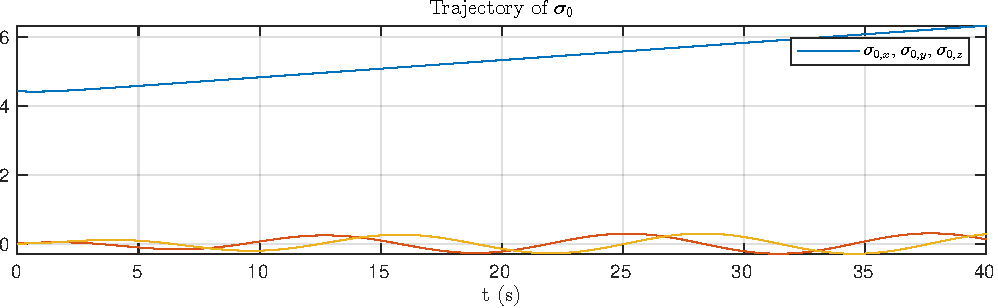
\includegraphics[width=\linewidth]{assets/plots/traj_xyz.pdf}
    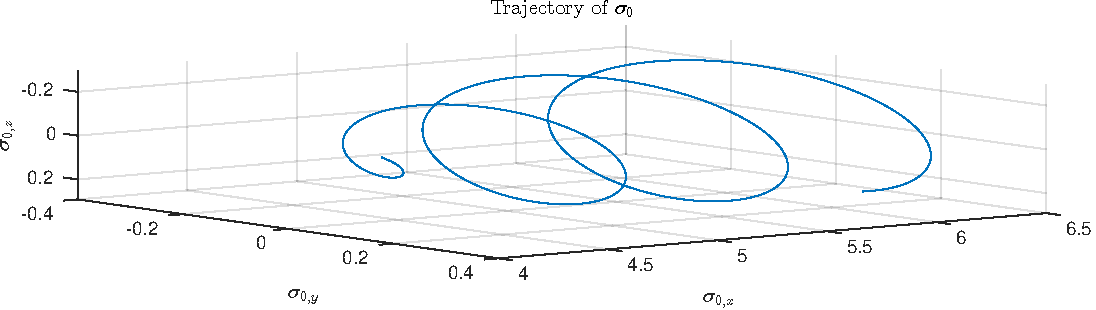
\includegraphics[width=\linewidth]{assets/plots/traj_taskspace.pdf}
    \caption{The desired task trajectory in the NED frame.}
    \label{fig:traj_f0}
\end{figure}

The task as seen in \autoref{fig:traj_f0} is the highest priority task.


\subsection{Control methods}
\subsubsection{Kinematic-level Control}

The kinematic-level control method used in the simulation is the velocity-level
controller presented in \autoref{sec:velocity_level_control}. As we are only considering
a case with two tasks, the question of successive versus augmented nullspace projections
are irrelevant. The projections used in the controller are inverse based
and the low-level joint-space controller chosen is a PD+ controller
with buoyancy/gravity compensation. Because of the simplicity of the shape of the robot,
these forces are relatively well known in a real-world scenario.

The gain matrices $\bm{K}_p$ and $\bm{K}_d$ as presented in \autoref{eq:Kp_Kd}
are chosen based on the assumption that the mass, Coreolis, damping and added mass
matrices are known, constant and diagonal. Under thesis assumption, the system model is approximated
as
\begin{align}
    \bar{\bm{M}}(\bm{0}) \ddot{\bm{q}} + \bar{\bm{C}}(\bm{0}, \dot{\bm{0}}) \dot{\bm{q}} +
    \bar{\bm{D}}(\bm{0}, \dot{\bm{0}}) \dot{\bm{q}} + \bm{g}(\bm{q}) \approx \bm{J}^T(\bm{q}) \bm{B} \bm{u},
\end{align}
where the bar denotes that the matrices are approximated. Using this approximation,
the system is decoupled and diagonal gain matrices can be chosen such that we get
a set of $n$ second-order systems with the same natural frequency and damping ratio.
In this case, the natural frequency is chosen as $\omega_n = \pi/6$ and the damping ratio
as $\zeta = 1$. Using this approximation, the gains are chosen as
\begin{subequations}
    \label{eq:kin:gains}
\begin{align}
    \bm{K}_p &= \operatorname{diag}\left(122, 206, 206, 0.5, 664.428, 664.428, 78, 78, 32, 32\right) \\
    \bm{K}_d &= \operatorname{diag}\left(306, 479, 479, 1, 1531, 1531, 195, 195, 65, 65\right).
\end{align}
\end{subequations}

The assumptions and implications of using gains based on the model are discussed
in \autoref{sec:simulation:results}.

\subsubsection{Dynamic-level Control}

The dynamic-level control method used in the simulation is the method presented in \autoref{sec:tpc:dynamic_level}. The forces $\bm{f}_t$ and $\bm{\tau}_t$ are computed using
a feedforward term and a PD controller. The gains of the PD controller are chosen
such that the feedback linearization controller renders the system as a second-order
system with a natural frequency of $\omega_n = \pi/6$ and a damping ratio of $\zeta = 1$.
This is done to make the comparison between the two controllers more fair. The forces
are computed as:
\begin{subequations}
\begin{align}
    \bm{f}_0^* = \ddot{\sigma}_0
    - 2 \zeta \omega_n \left(\dot{\bm{f}}_0(\bm{q}) - \dot{\bm{\sigma}}_0(t)\right)
    - \omega_n^2 \left(\bm{f}_0(\bm{q}) - \bm{\sigma}_0(t)\right) \\
    \bm{f}_1^* = \ddot{\sigma}_1
    - 2 \zeta \omega_n \left(\dot{\bm{f}}_1(\bm{q}) - \dot{\bm{\sigma}}_1(t)\right)
    - \omega_n^2 \left(\bm{f}_1(\bm{q}) - \bm{\sigma}_1(t)\right)
\end{align}
\end{subequations}
Because of the two tasks being incompatible at some point, the $\bm{\Lambda}_{p|t}$
matrix can not be computed using an ordinary inverse, as this will give numerical issues.
Instead, different methods of damped pseudoinverses presented in \autoref{sec:tpc:sing_robust}
are used. The parameters and the specific method used are presented in \autoref{sec:simulation:results}.

The damped pseudoinverses that are used are
\begin{itemize}
    \item Least squares (LS).
    \item Damped least squares (DLS) with $\lambda = 0.1$.
    \item Variable damped least squares (VDLS) with $\lambda = 0.1$ and $\epsilon = 0.1$.
\end{itemize}
Details are presented in in \autoref{sec:tpc:sing_robust}.

\subsection{Simulation Environment}

The initial state of the robot in the simulation are given in \autoref{tab:initial}.
The state was chosen such that it satisfies task $1$, for the tail,
but not task $0$, the trajectory tracking task. This was done to show convergence
to the task when having an error in the initial conditions. The initial state
can be seen in \autoref{tab:initial} and \autoref{fig:init_pos}. The initial velocity
is set to $\bm{0}$. The figure
shows the position of the three links as well as their orientation as visualized
by the red, green and blue arrows symbolizing the $x$, $y$ and $z$ axes of the
links.
\begin{table}[h!]
    \centering
    \begin{tabular}{|c|c|c|c|c|c|c|c|c|c|c|c|}
        \hline
        Parameter & $x^n$ & $y^n$ & $z^n$ & $\phi$ & $\theta$ & $\psi$ & $a_1$ & $a_2$ & $a_3$ & $a_4$ \\ \hline
        Value & 3.17 & 0 & -1.0 & 0 & 0 & 0 & -0.59 & 0 & -0.88 & 0 \\ \hline
        Unit & m & m & m & rad & rad & rad & rad & rad & rad & rad \\
        \hline
    \end{tabular}
    \caption{Initial conditions for the Eelume 500 robot in simulation.}
    \label{tab:initial}
\end{table}

\begin{figure}[h]
    \centering
    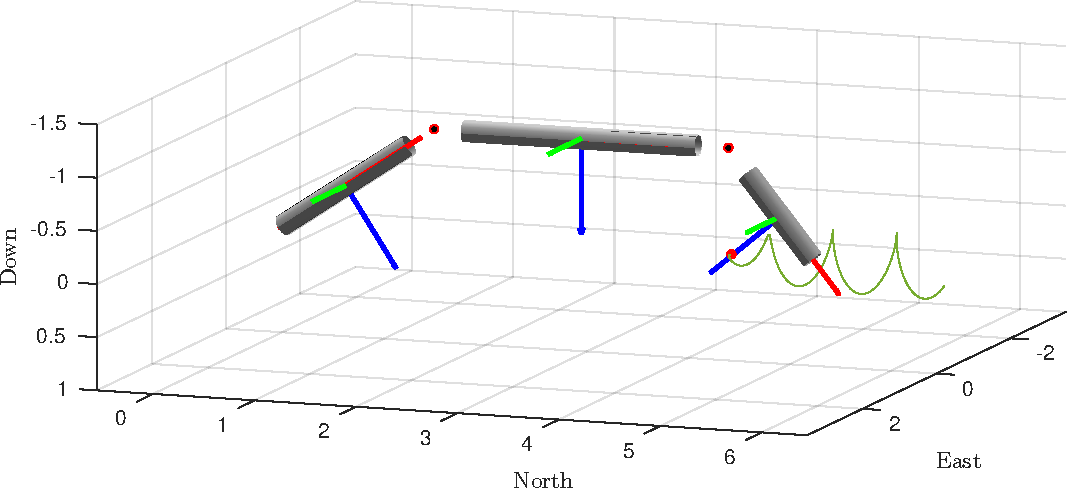
\includegraphics[width=\linewidth]{assets/plots/initial_pos.pdf}
    \caption{The initial position of the robot in the NED frame.}
    \label{fig:init_pos}
\end{figure}
The time step of the simulation is $\Delta t = 0.01$ [s]. The controller is
called at every time step. The controllers all give a desired input $\bm{u}$ which
maps to a specific torque in joint motors and a force in the thrusters.
This means that the controllers will have to do the inverse mapping, which
is a relatively simple operation as the \pymuvs package provides this inverse
mapping by default. All of
the forces and torques are limited to a maximum of $100$ N and $100$ Nm, respectively.
These limitations are quite high compared to the Eelume 500 robot, but are chosen
such that it is apparent when the controllers are saturating. The forces and torques
are "pass through", meaning that the forces and torques are directly applied without
any filtering.

\subsection{Performance Metrics}
The following performance metrics will be considered when comparing the two controllers:

\textbf{Task error}: We define the task error as the two-norm of the difference
between the desired task position and the actual task position. The task error
is computed for both tasks.
\begin{align}
    \bm{e}_i &:= ||\bm{f}_i(\bm{q}) - \bm{\sigma}_i(t)||_2 &
        i &= 0, 1.
\end{align}

\textbf{Computation time}: The time it takes to compute the control input at each
time step will be measured. This is done to see if it is feasible to implement the
two controllers on a real-world system. Note that the simulation time also includes
simulation of the dynamics and saving of data. Furthermore, the implementation is
not written with performance in mind, it will however give an indication of the
computational cost of the two controllers.

\textbf{Thruster usage}: If some controllers give a higher thruster usage than others
will give an indication of how realistic the controllers are. Considering the
pseudo-inverse used in both controllers, having a high and fast varying thruster
usage can be a sign of numerical instability.

\textbf{Joint torque usage}: Equally to the thruster usage, the joint torque usage
will give an indication of how realistic the controllers are. Too high or too
fast varying joint torques can be a sign of numerical instability.

% -----------------------------------------------------------------------------

% -----------------------------------------------------------------------------
\newpage
\section{Results and Discussion}
\label{sec:simulation:results}

% -----------------------------------------------------------------------------
\subsection{Kinematic-level Control}

The following subsection presentes the result of the simulation using the
kinematic level controller.

\subsubsection{Task error}

The task error for this controller are presented in \autoref{fig:kin:task_error}.
One can see that the controller struggles to complete both tasks simultaneously,
and that the task error for task $0$ is generally higher than that of task $1$.
From \autoref{fig:kin:task_error}, one can see that there is some time delay
when tracking the desired velocity. Furthermore, the implemented controller
struggles to track the desired roll rate. Some snapshots of the position of the
robot are shown in \autoref{fig:kin:vis}. This figure clearly shows that the
robot starts off by adjusting the position as to satisfy both tasks. It is evident
that it is not able to track both tasks perfectly. At the end of the simulation,
a clear prioritization of task $0$ is seen, as well as a change in the roll angle.

\begin{figure}[h!]
    \centering
    \includegraphics[page=2,width=\linewidth]{assets/results/kinematic/h5data.pdf}
    \caption{Task space error using kinematic-level control.}
    \label{fig:kin:task_error}
\end{figure}
\begin{figure}[h!]
    \centering
    \includegraphics[page=9,width=\linewidth]{assets/results/kinematic/plot.pdf}
    \includegraphics[page=10,width=\linewidth]{assets/results/kinematic/plot.pdf}
    \caption{Desired and actual velocities using kinematic-level control.}
    \label{fig:kin:vel_des}
\end{figure}
\begin{figure}[h!]
    \centering
    \begin{subfigure}[b]{0.45\linewidth}
        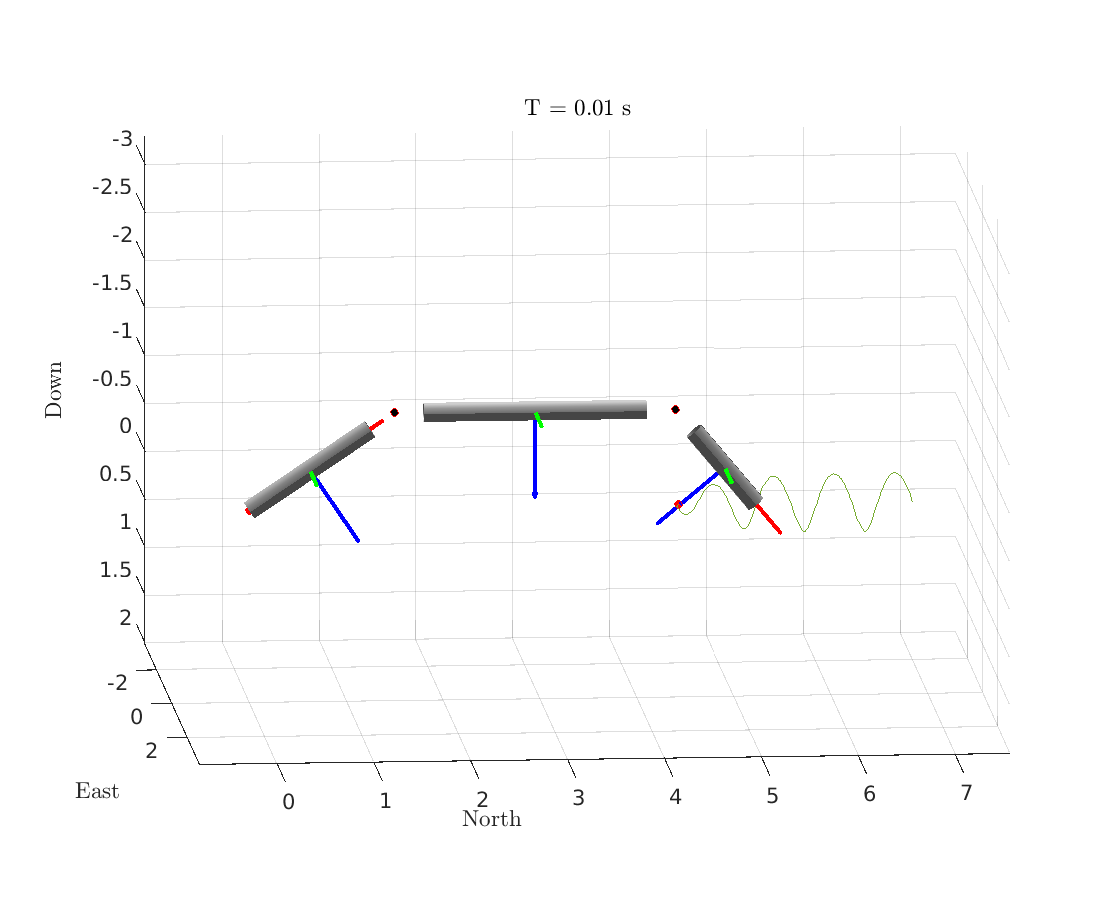
\includegraphics[page=1,width=\linewidth]{assets/results/kinematic/gif.pdf}
    \end{subfigure}
    \begin{subfigure}[b]{0.45\linewidth}
        \includegraphics[page=2,width=\linewidth]{assets/results/kinematic/gif.pdf}
    \end{subfigure}
    \begin{subfigure}[b]{0.45\linewidth}
        \includegraphics[page=3,width=\linewidth]{assets/results/kinematic/gif.pdf}
    \end{subfigure}
    \begin{subfigure}[b]{0.45\linewidth}
        \includegraphics[page=4,width=\linewidth]{assets/results/kinematic/gif.pdf}
    \end{subfigure}
    \begin{subfigure}[b]{0.45\linewidth}
        \includegraphics[page=5,width=\linewidth]{assets/results/kinematic/gif.pdf}
    \end{subfigure}
    \begin{subfigure}[b]{0.45\linewidth}
        \includegraphics[page=6,width=\linewidth]{assets/results/kinematic/gif.pdf}
    \end{subfigure}
    \caption{Visualisation of the position of the robot using kinematic-level control.}
    \label{fig:kin:vis}
\end{figure}

\subsubsection{Computation Time}

The computation time for the kinematic-level controller is presented in \autoref{fig:kin:comp_time}
and \autoref{tab:kin:comp_time}. The computation time is relatively low, with a mean of $22.5$ $\mu$s.
and a standard deviation of $2.4$ $\mu$s. There are some outliers in \autoref{fig:kin:comp_time},
showing that the computation time can be up to approximately $5$ times higher than the mean
for a few time steps during the simulation.

\begin{figure}[h!]
    \centering
    \includegraphics[page=3,width=\linewidth]{assets/results/kinematic/h5data.pdf}
    \caption{Computation time at each time-step using kinematic-level control.}
    \label{fig:kin:comp_time}
\end{figure}
\begin{table}[h!]
    \centering
    \begin{tabular}{|c|c|}
        \hline
        Mean & Standard Deviation \\ \hline
        22.5 $\mu$s & 2.4 $\mu$s \\ \hline
    \end{tabular}
    \caption{Computation time using kinematic-level control.}
    \label{tab:kin:comp_time}
\end{table}

\subsubsection{Thruster and Joint Torque Usage}
\autoref{fig:kin:forces} shows the forces and torques applied to the robot by the
motors and thrusters. All the torques have an absolute value of less than $30$ Nm,
with significantly lower values after the first couple of seconds. One observes
that the forces are smooth and do not have any large spikes or discontinuities.
The same can be said for the thruster forces, wich all have an absolute value of less
than $50$ Nm.
\begin{figure}[h!]
    \centering
    \includegraphics[page=7,width=\linewidth]{assets/results/kinematic/plot.pdf}
    \includegraphics[page=8,width=\linewidth]{assets/results/kinematic/plot.pdf}
    \caption{Forces and torques applied to the robot using kinematic-level control.}
    \label{fig:kin:forces}
\end{figure}


\iffalse
\begin{figure}[h!]
    \centering
    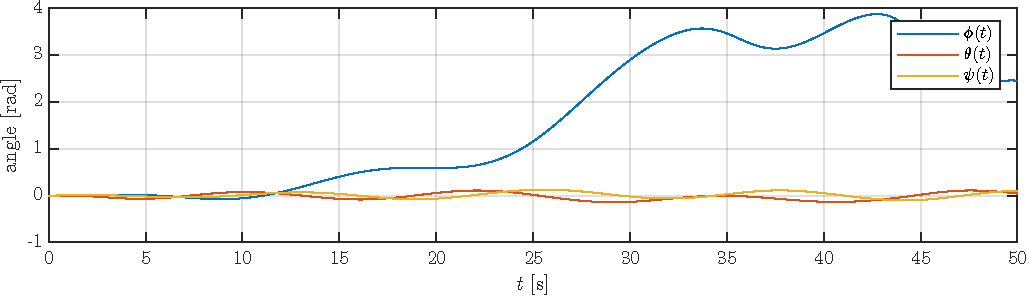
\includegraphics[page=1,width=\linewidth]{assets/results/kinematic/plot.pdf}
    \includegraphics[page=2,width=\linewidth]{assets/results/kinematic/plot.pdf}
    \includegraphics[page=3,width=\linewidth]{assets/results/kinematic/plot.pdf}
    \includegraphics[page=6,width=\linewidth]{assets/results/kinematic/plot.pdf}
    \includegraphics[page=4,width=\linewidth]{assets/results/kinematic/plot.pdf}
    \includegraphics[page=5,width=\linewidth]{assets/results/kinematic/plot.pdf}
    \caption{Positions and velocities of the robot in the NED frame using kinematic-level control.}
\end{figure}
\fi

\FloatBarrier
% -----------------------------------------------------------------------------
\subsection{Dynamic-level Control}

The following subsection presents the result of the simulation ising the dynamic-level
controller. The controller is used with the VDLS pseudoinverse method. A comparison
of the different pseudoinverse methods is presented later in this section.

\subsubsection{Task Error}
The task error can be seen in \autoref{fig:dyn:error}. The task error for task $0$
starts off high, as expected, but quickly moves towards zero. the $1$ task error
is generally higher than that of task number $0$. Expecially towards the end of the
simulation. An illustration of the position at specific time steps can be seen in
\autoref{fig:dynamic_vis}. One can see that the robot is able to track both tasks
in the beginning of the simulation. As fullfilling both tasks becomes impossible,
there is a clear prioritization of task $0$ over task $1$.

\begin{figure}[h!]
    \centering
    \includegraphics[page=2,width=\linewidth]{assets/results/dynamic/h5data.pdf}
    \caption{Task space error using dynamic-level control.}
    \label{fig:dyn:error}
\end{figure}

\begin{figure}[h!]
    \centering
    \begin{subfigure}[b]{0.45\linewidth}
        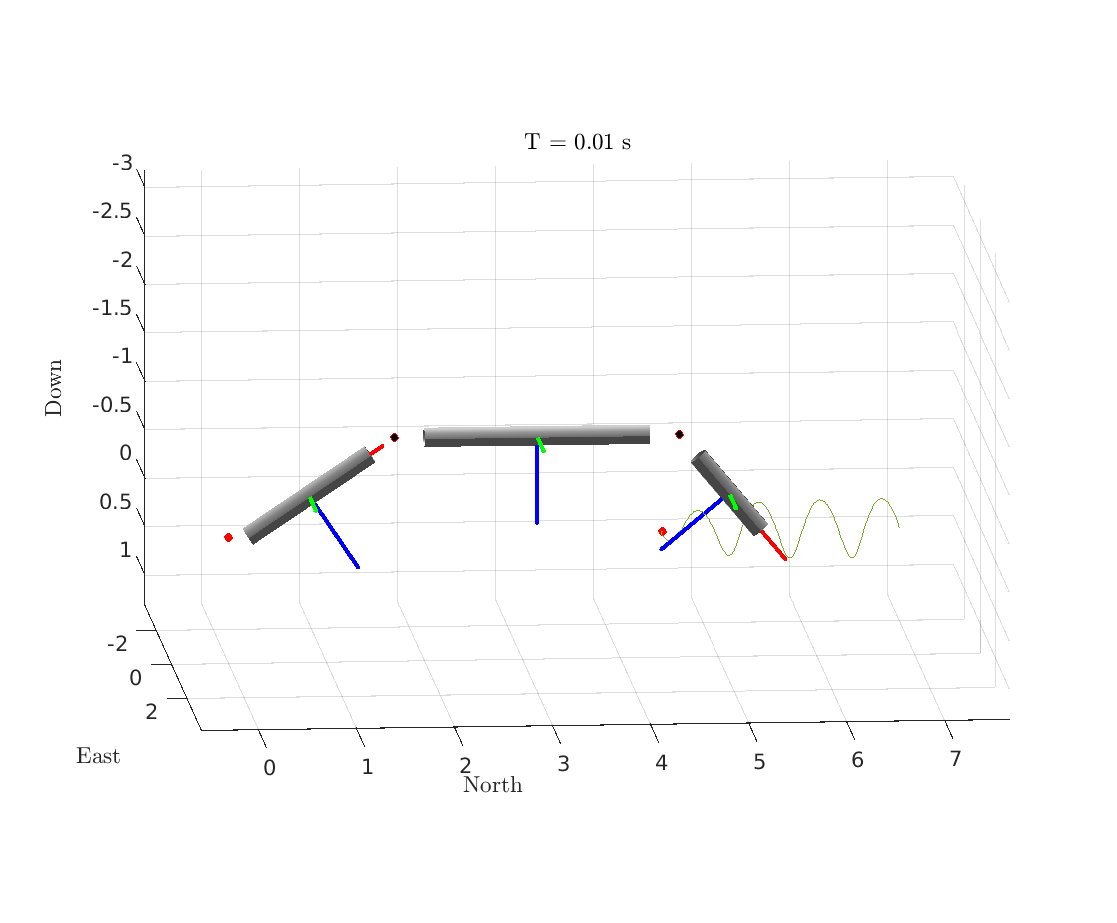
\includegraphics[page=1,width=\linewidth]{assets/results/dynamic/gif.pdf}
    \end{subfigure}
    \begin{subfigure}[b]{0.45\linewidth}
        \includegraphics[page=2,width=\linewidth]{assets/results/dynamic/gif.pdf}
    \end{subfigure}
    \begin{subfigure}[b]{0.45\linewidth}
        \includegraphics[page=3,width=\linewidth]{assets/results/dynamic/gif.pdf}
    \end{subfigure}
    \begin{subfigure}[b]{0.45\linewidth}
        \includegraphics[page=4,width=\linewidth]{assets/results/dynamic/gif.pdf}
    \end{subfigure}
    \begin{subfigure}[b]{0.45\linewidth}
        \includegraphics[page=5,width=\linewidth]{assets/results/dynamic/gif.pdf}
    \end{subfigure}
    \begin{subfigure}[b]{0.45\linewidth}
        \includegraphics[page=6,width=\linewidth]{assets/results/dynamic/gif.pdf}
    \end{subfigure}
    \caption{Visualisation of the position of the robot using dynamic-level control.}
    \label{fig:dynamic_vis}
\end{figure}

\subsubsection{Computation Time}

The computation time for the dynamic-level controller is presented in \autoref{fig:dyn:comp_time}
and \autoref{tab:dyn:comp_time}. The computation time is relatively low, with a mean of $48.5$ $\mu$s
and a standard deviation of $3.4$ $\mu$s. There are some outliers in \autoref{fig:dyn:comp_time},
reaching values of up to $170$ $\mu$s.

\begin{table}[h!]
    \centering
    \begin{tabular}{|c|c|}
        \hline
        Mean & Standard Deviation \\ \hline
        48.5 $\mu$s & 3.4 $\mu$s \\ \hline
    \end{tabular}
    \caption{Computation time using dynamic-level control.}
    \label{tab:dyn:comp_time}
\end{table}

\begin{figure}[h!]
    \centering
    \includegraphics[page=3,width=\linewidth]{assets/results/dynamic/h5data.pdf}
    \caption{Computation time at each time-step using dynamic-level control.}
    \label{fig:dyn:comp_time}
\end{figure}

\subsubsection{Thruster and Joint Torque Usage}

The forces and torques applied to the robot by the motors and thrusters are presented
in \autoref{fig:dyn:forces}. The joint torques stars of low in amplitude, reaching no more than
approximately $7$ Nm. They do however somewhat high frequency content. The same can be said
for the thruster forces. They start of low in amplitude and reach no more than approximately
$10$ N of force. Similarly to the torques, they have a somewhat high frequency content.

\begin{figure}[h!]
    \centering
    \includegraphics[page=7,width=\linewidth]{assets/results/dynamic/plot.pdf}
    \includegraphics[page=8,width=\linewidth]{assets/results/dynamic/plot.pdf}
    \caption{Forces and torques applied to the robot using dynamic-level control.}
    \label{fig:dyn:forces}
\end{figure}

\subsubsection{Pseudoinverse Methods}

The results of the simulation using the different pseudoinverse methods are presented
in \autoref{fig:ls}, \autoref{fig:dls} and \autoref{fig:vdls}. We observe that the
VDLS- and DLS-pseudoinverse methods are very similar in terms of both task error and
singular values of the Jacobian. The LS-pseudoinverse method, however, gives a much
better results in terms of task error. The singular values using this method are
also much lower than the other two methods, being as low as $0.05$.

Looking at the desired forces outputed by the controllers in \autoref{fig:ls_vdls_force},
one can see that the VDLS-pseudoinverse gives a much smoother force output compared
to the LS-pseudoinverse. The point at which the forces applied by the LS-pseudoinverse
controller are much higher coencides with the time interval where the singular values
are low in \autoref{fig:ls}. The forces applied using the LS-psuedoinverse reaches
a maximum of $100$ N, which is the maximum force allowed in the simulation.

\begin{figure}[h!]
    \centering
    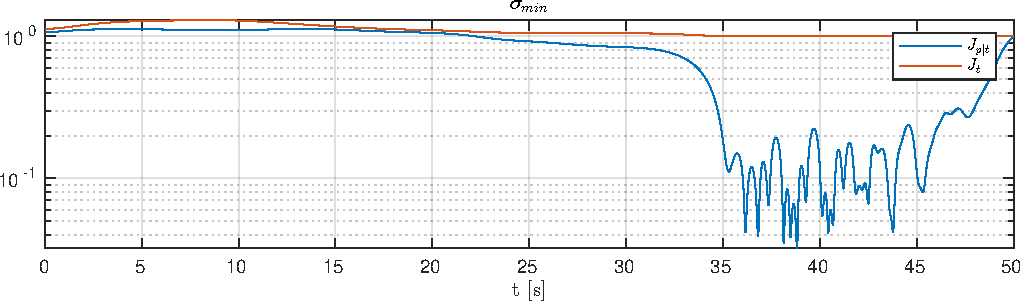
\includegraphics[page=1,width=\linewidth]{assets/results/LSI.pdf}
    \includegraphics[page=2,width=\linewidth]{assets/results/LSI.pdf}
    \caption{Task space error and singular values using LS pseudoinverse.}
    \label{fig:ls}
\end{figure}

\begin{figure}[h!]
    \centering
    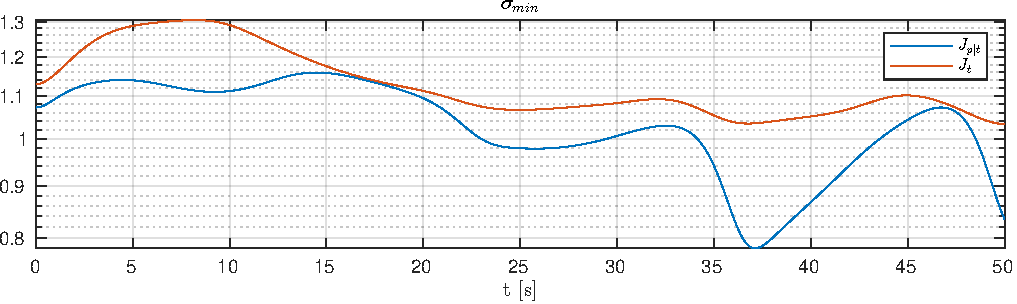
\includegraphics[page=1,width=\linewidth]{assets/results/DLSI.pdf}
    \includegraphics[page=2,width=\linewidth]{assets/results/DLSI.pdf}
    \caption{Task space error and singular values using DLS pseudoinverse.}
    \label{fig:dls}
\end{figure}

\begin{figure}[h!]
    \centering
    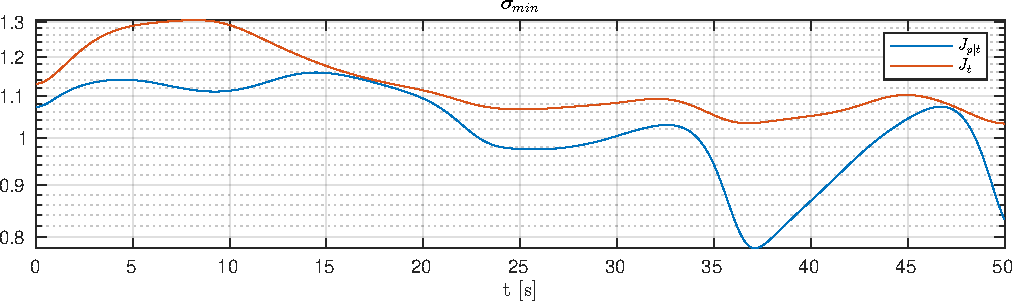
\includegraphics[page=1,width=\linewidth]{assets/results/VDLSI.pdf}
    \includegraphics[page=2,width=\linewidth]{assets/results/VDLSI.pdf}
    \caption{Task space error and singular values using VDLS pseudoinverse.}
    \label{fig:vdls}
\end{figure}

\begin{figure}[h!]
    \centering
    \begin{subfigure}[b]{\linewidth}
        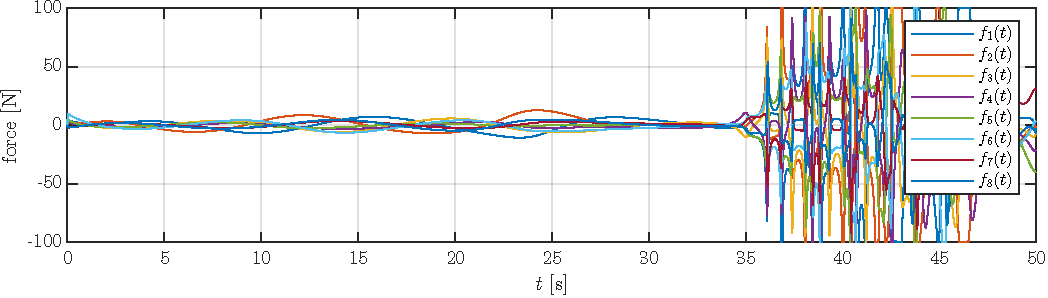
\includegraphics[page=1,width=\linewidth]{assets/ls_vdls_force.pdf}
        \caption{Forces using dynamic-level control with LS pseudoinverse.}
    \end{subfigure}
    \begin{subfigure}[b]{\linewidth}
        \includegraphics[page=2,width=\linewidth]{assets/ls_vdls_force.pdf}
        \caption{Forces using dynamic-level control with VDLS pseudoinverse.}
    \end{subfigure}
    \caption{Comparison of forces using LS and VDLS pseudoinverse.}
    \label{fig:ls_vdls_force}
\end{figure}

% -----------------------------------------------------------------------------
\FloatBarrier
\subsection{Discussion}

\subsubsection{Kinematic-level Control}

Using the dynamic-level controller we observe in \autoref{fig:kin:task_error} that
the task space error is fluctuating and relatively high. Using the framework derived
in \autoref{sec:tpc} we would expect perfect tracking of the task, under the assumption
that we can track the desired joint velocities, meaning $\bm{q}(t) = \bm{q}_d(t)$.
From \autoref{fig:kin:vel_des} we see that the desired velocities are tracked,
but that there is some time delay in the tracking. This is expected, and is due
to the fact that we are using a PD+ with no feedforward term to track the desired
joint velocities. This creates a time delay in the tracking, making the task space
errors non-zero.

In \autoref{fig:kin:task_error} we see that the time delay in the tracking of the
reference velocities are similar across all variables, except for the roll angle.
Looking at the chosen gains from \autoref{eq:kin:gains} we observe that the fourth
entry in the gain matrix is very low compared to the other gains. This is a result
of the way the gains are chosen. There might be some large copling terms in the
dynamics that are not accounted for when choosing gains from the diagonalized
approximation of the system. Choosing a different method of choosing the gains
and spending more time on tuning the controller might give better results. This
might also explain why we see a change in the roll angle at the last time
step in \autoref{fig:kin:vis}. The controller is not able to track the desired
roll rate, affecting the roll angle.

The average computation time, as presented in \autoref{tab:kin:comp_time}, is very low.
This is a very good indication that the controller can be implemented on a physical
system. The standard deviation is also very low, meaning that the computation time
is relatively stable. The outliers in \autoref{fig:kin:comp_time} might be due to
the computer interrupting the process, or some other external factor. It is important
to note that the simulator was not run in a real-time environment, meaning that
inconsistencies in the computation time are to be expected.

The forces and torques applied to the robot are presented in \autoref{fig:kin:forces}.
All of the values are reasonable, and the forces are very smooth. This is a good
indication that the controller is suited for a physical system, where thrust limitations
and thruster dynamics are important to consider. Overall, the kinematic-level controller
performs okay, but there is room for improvement. The high task space error is
concerning, and the controller is not able to track the desired roll rate needs
to be addressed. These problems may however be solved by spending more time finding
a good lower-level controller and tuning the gains of this controller.

\subsubsection{Dynamic-level Control}

\autoref{fig:dyn:error} shows the task error when using the VDLS pseudoinverse.
It shows a promising convergence of the primary task, task $0$. Even after the
fulfilling both tasks become impossible, the error for the primary task stays
relatively constant. It is a bit interesting that the tracking of task $1$ is
relatively poor. This can be due to the fact that the VDLS pseudo-inverse is used
instead of a proper inverse. This will be discussed in more detail when comparing
pseudoinverse methods later in this chapter.

In \autoref{tab:dyn:comp_time} we can see the computation time for the dynamic-level
controller. It has a relatively stable computation time, with a mean of $48.5$ $\mu$s
and a standard deviation of $3.4$ $\mu$s. This is well within the limits of what
is required for a physical system. The outliers in \autoref{fig:dyn:comp_time},
as mentioned earlier, might be due to the computer interrupting the process.

\autoref{fig:dyn:forces} shows that the forces and torques computed by the controller
are reasonable in amplitude, but have a somewhat high frequency content. Although
not too high, this might cause problem for a physical system with thruster dynamics,
where the thrusters might not be able to keep up with the high frequency content.
Physical tests are needed to determine if the controller is feasible for a real-world
system.

When comparing the different pseudoinverse methods in \autoref{fig:vdls} and
\autoref{fig:dls}, we see that the VDLS and DLS methods give very similar results.
This can be explained by looking at \autoref{fig:1_x}. Notice that the VDLS and
DLS give very similar singular values. This explains why the task error is similar
for the two methods. The LS method, however, gives a much better result in terms
of task error. This can be explained by looking at the smallest singular value
of the Jacobian in the same graph. We see that the singular values are much lower
in a time interval after approximately $35$ seconds. This will imply greater
forces and torques, as the mass matrix, a function of the Jacobian, is inverted.
This is also observed in \autoref{fig:ls_vdls_force}, where very high and oscillating
forces are shown. The observed difference in error can therefore be explained by
the accuracy of the inverses. The LS method gives much better results in terms of
task error, but the forces and torques are not realistic. The VDLS and DLS methods
give more realistic forces and torques, but the task error is higher. This is a
trade-off that needs to be considered when choosing a pseudoinverse method.

\subsection{Comparative Analysis}

Comparing the two controllers we observe that the kinematic-level controller has
a higher task error than the dynamic-level controller. This can in part be explained
by the fact that the kinematic-level controller
is dependent on a lower-level joint controller, which might not be able to track
the desired velocities. Coupling terms between the kinematic and dynamic levels
will affect the performance of the kinematic-level controller. The dynamic level controller
commands forces which are a bit lower in amplitude, especially in the beginning,
but have a higher frequency content than the dynamic-level controller. 

The kinematic-level controller has a lower computation time than the dynamic-level.
\autoref{tab:kindyn:comp_time} shows that the kinematic-level controller has about
half the computation time of the dynamic-level controller. It can be argued that
this does not matter, as both controllers run at a frequency so high that they
are both fit for real-time implementations.
\begin{table}[h]
    \centering
    \begin{tabular}{|c|c|c|}
        \hline
        Controller & Mean & Standard Deviation \\ \hline
        Kinematic & 22.5 $\mu$s & 2.4 $\mu$s \\
        Dynamic & 48.5 $\mu$s & 3.4 $\mu$s \\ \hline
    \end{tabular}
    \caption{Computation time for the two controllers.}
    \label{tab:kindyn:comp_time}
\end{table}

Using the LS pseudoinverse, the dynamic-level controller gives the best results.
This is however at the cost of realistic forces and torques. The VDLS and DLS
give more realistic thruster and joint torques, but the task error is higher. Overall,
the VDLS and DLS methods are more suited for a real-world scenario, and will
probably give better results in practice.

From the simulation study, it seems like the dynamic-level controller is more
suitable for controlling the Eelume 500 robot. It has a lower task error, reasonable
forces and torques, and the computation time is still low enough for real-time
implementations.An important unanswered question still remains; how well does the
dynamic-level controller perform when the model is inaccurate? This is a question
that needs to be answered in order to truly determine the which controller is best.
